\documentclass[conference]{IEEEtran}
\IEEEoverridecommandlockouts
% The preceding line is only needed to identify funding in the first footnote. If that is unneeded, please comment it out.
\usepackage{cite}
\usepackage{amsmath,amssymb,amsfonts}
\usepackage{algorithmic}
\usepackage{graphicx}
\usepackage{textcomp}
\usepackage{xcolor}
\usepackage{background}

\backgroundsetup{contents=FAKE}

\def\BibTeX{{\rm B\kern-.05em{\sc i\kern-.025em b}\kern-.08em
    T\kern-.1667em\lower.7ex\hbox{E}\kern-.125emX}}
\begin{document}

\title{Archangel protocol for pedestrian to vehicle communication via 5G networks\\}

\makeatletter
\newcommand{\linebreakand}{
    \end{@IEEEauthorhalign}
    \hfill\mbox{}\par
    \mbox{}\hfill\begin{@IEEEauthorhalign}
}
\makeatother

\author{\IEEEauthorblockN{1\textsuperscript{st} Dávid Rammer}
    \IEEEauthorblockA{\textit{Eötvös Loránd University} \\
        \textit{Computer Science}\\
        Budapest, Hungary \\
        rwauyx@inf.elte.hu}
    \and
    \IEEEauthorblockN{2\textsuperscript{nd} Gergő Tanai}
    \IEEEauthorblockA{\textit{Eötvös Loránd University} \\
        \textit{Computer Science}\\
        Budapest, Hungary \\
        dfnx0d@inf.elte.hu}
    \and
    \IEEEauthorblockN{3\textsuperscript{rd} Patrik Szalai}
    \IEEEauthorblockA{\textit{Eötvös Loránd University} \\
        \textit{Computer Science}\\
        Budapest, Hungary \\
        bzckg6@inf.elte.hu}
    \linebreakand
    \IEEEauthorblockN{4\textsuperscript{th} Szandra Ladányi}
    \IEEEauthorblockA{\textit{Eötvös Loránd University} \\
        \textit{Computer Science}\\
        Budapest, Hungary \\
        uxqurt@inf.elte.hu}
    \and
    \IEEEauthorblockN{5\textsuperscript{th} Tomás Varga}
    \IEEEauthorblockA{\textit{Eötvös Loránd University} \\
        \textit{Computer Science}\\
        Budapest, Hungary \\
        yi4i0v@inf.elte.hu}
}

\maketitle

\begin{abstract}
    Everyone can see that there are more and more self-driving cars on the roads. Human supervision is becoming less and less necessary behind the wheel, but this can pose a great danger to other drivers and pedestrians. But we know, that nowadays nearly everyone has their smartphones in their pockets. To increase their safety, we use it to our advantage so that smartphones send their specific location and other traffic-relevant data indirectly to self-driving cars nearby. However, this is such a large amount of data movement that 4G networks would be insufficient, so we would use 5G networks. Thus, the Archangel protocol we have created helps communication over 5G networks to ensure that the data can be transmitted from sender to receiver as the transfer of this data increases pedestrian safety.
\end{abstract}

\begin{IEEEkeywords}
    protocol, P2V, self-driving cars, pedestrian safety, transport
\end{IEEEkeywords}

\section{Introduction}
Autonomous driving, and therefore self-driving cars have a growing interest around the world. It is a brilliant improvement to modern vehicles. There are already some autonomous systems, but a human driver must supervise its operation at all times. They can do it either remotely or by sitting at the wheel and intervening when they see it needed.

Although it is still the future that self-driving vehicles will populate the roads, precautions have to be made already to make these systems as safe as possible. Many sensors, cameras, lidars and other systems are placed in these vehicles to prevent accidents. But these vehicles won't be the only ones on the streets. There will be other cars with drivers, motionless objects. The cars' systems are ready to detect and avoid them. But what about the pedestrians? In case of an accident, they can be in even more danger than those sitting in the car. Are the self-driving cars' systems enough to ensure their safety too?

In today's society, most people have a smartphone in their pocket at all times. Based on this fact, it is possible to create some security layers in the self-driving cars' system solely for pedestrians' safety. For this, self-driving cars and smartphones need to communicate with each other. \cite{b1}

Self-driving cars are dealing with huge amounts of data. The surrounding objects, people, the road, other cars etc. This data has to move quickly and has to reach the destination reliably.

Currently the protocols are for the 4G networks which are way slower than the upcoming 5G. It could become insufficient in the near future. That's why it is mandatory to make new protocols for the 5G networks.

5G uses beamforming which means it's not spreading the data everywhere, but concentrates it to the destinations. The problem with spreading the data is that the strength of the signal decreases cubically. With 5G delivering up to 20 Gigabits of data per second became possible.
We used this possibility with the Archangel protocol, that's why it is faster and more reliable than the old ones.

Self-driving cars that are using this protocol can transfer/receive data faster and more reliably to/from other cars or pedestrians' phones. This means that these cars have more information about their surroundings so they can operate safer.

\section{State of the art}
Because of the limitations of the third generation (3G) cellular network, the first self-driving cars couldn’t use it to achieve the ‘Vehicle to everything’ (V2X) communication so the initial implementation used IEEE 802.11p  which is a standard based on Wi-Fi technology. The IEEE's WAVE, or Wireless Access for Vehicular Environments program has been running in the unlicensed 5.9GHz frequency band and provided short-range (under 1km), low latency ($ \sim $2ms) and high reliability according to the US Department of Transportation. This was able to work in high vehicle speed mobility conditions and delivers performance immune to extreme weather conditions (e.g. rain, fog, snow etc.). The only problem was it couldn’t handle longer distances that cellular networks can provide. The introduction of the Long-Term Evolution (LTE) fourth-generation (4G) wireless standard, which increased network capacity and speed, has provided an excellent foundation for the ‘Cellular vehicle to everything’ (C-V2X) communication method. Its key advantage is that it has two operational modes.

\begin{enumerate}
    \item The first is low-latency C-V2X Direct Communications over the PC5 interface on the unlicensed 5.9GHz band (which is technically the same as before). This is designed for active safety messages such as immediate road hazard warnings and other short-range ‘Vehicle to vehicle’ (V2V), ‘Vehicle to infrastructure’ (V2I), and ‘Vehicle to pedestrians’ (V2P) situations.
    \item The second mode is communications over the Uu interface on the LTE cellular network, and can handle ‘Vehicle to Network’ (V2N) use cases like infotainment and latency-tolerant safety messages concerning longer-range road hazards or traffic conditions. Because it doesn't use cellular connectivity, IEEE 802.11p can only match this mode by making ad hoc connections to roadside base stations. \cite{b2}
\end{enumerate}

As far as LTE goes, this technology can’t handle intense data pressure through the network thus the whole system needs the most current cellular network, which is 5G in this case.

IEEE 802.11p has the advantage of earlier development and deployment. On the other, hand C-V2X offers arguably better performance as well as safer assisted and autonomous driving.

Although the standards debate is in full flow around the world, testing and even product implementation is now underway in some regions.

In March 2019, the European Commission put forward legislation favouring the IEEE 802.11p based ITS-G5 over C-V2X. This prompted activity from the C-V2X-supporting GSMA, arguing that 802.11p “is not a future-proof, is a standalone technology and cannot be integrated into 4G or 5G networks”. The European legislation is currently preparing for another vote.

The US has proven to be fertile ground for 802.11p-based DSRC (Dedicated Short-Range Communications) up to 2018. However,  as in Europe, the rise of C-V2X as an alternative to the IEEE 802.11p is causing US regulators and car manufacturers to reconsider their positions.

China is a leading supporter of C-V2X with LTE-based solutions, even running a city-wide LTE-V2X pilot project in Wuxi. Ford has announced plans to deploy C-V2X technology in China in 2021.

5G already uses beamforming, which technically the application of multiple radiating elements transmitting the same signal at an identical wavelength and phase, which combine to create a single antenna with a longer, more targeted stream which is formed by reinforcing the waves in a specific direction. \cite{b3}

\section{The Archangel protocol}
Our proposal is to define a new, extremely reliable Pedestrian to Vehicle (P2V) communication protocol, called Archangel protocol, the advantages of which can be used to provide an extra layer of protection for pedestrians in the vicinity of self-driving cars.

In our solution we are taking the advantage of the 5G cellular network \cite{b4,b5}, which has continuously increasing coverage, such as extraordinarily high bandwidth, low latency and the beamforming technology introduced with it. These are the qualities that make it possible to use the cellular network for transferring the data safely between devices involved in traffic situations. As a result of this, removing the restrictions on direct forms of communication between cars. For example, the case of a street corner with thick, signal-blocking walls.

\begin{figure}[h]
    \centering
    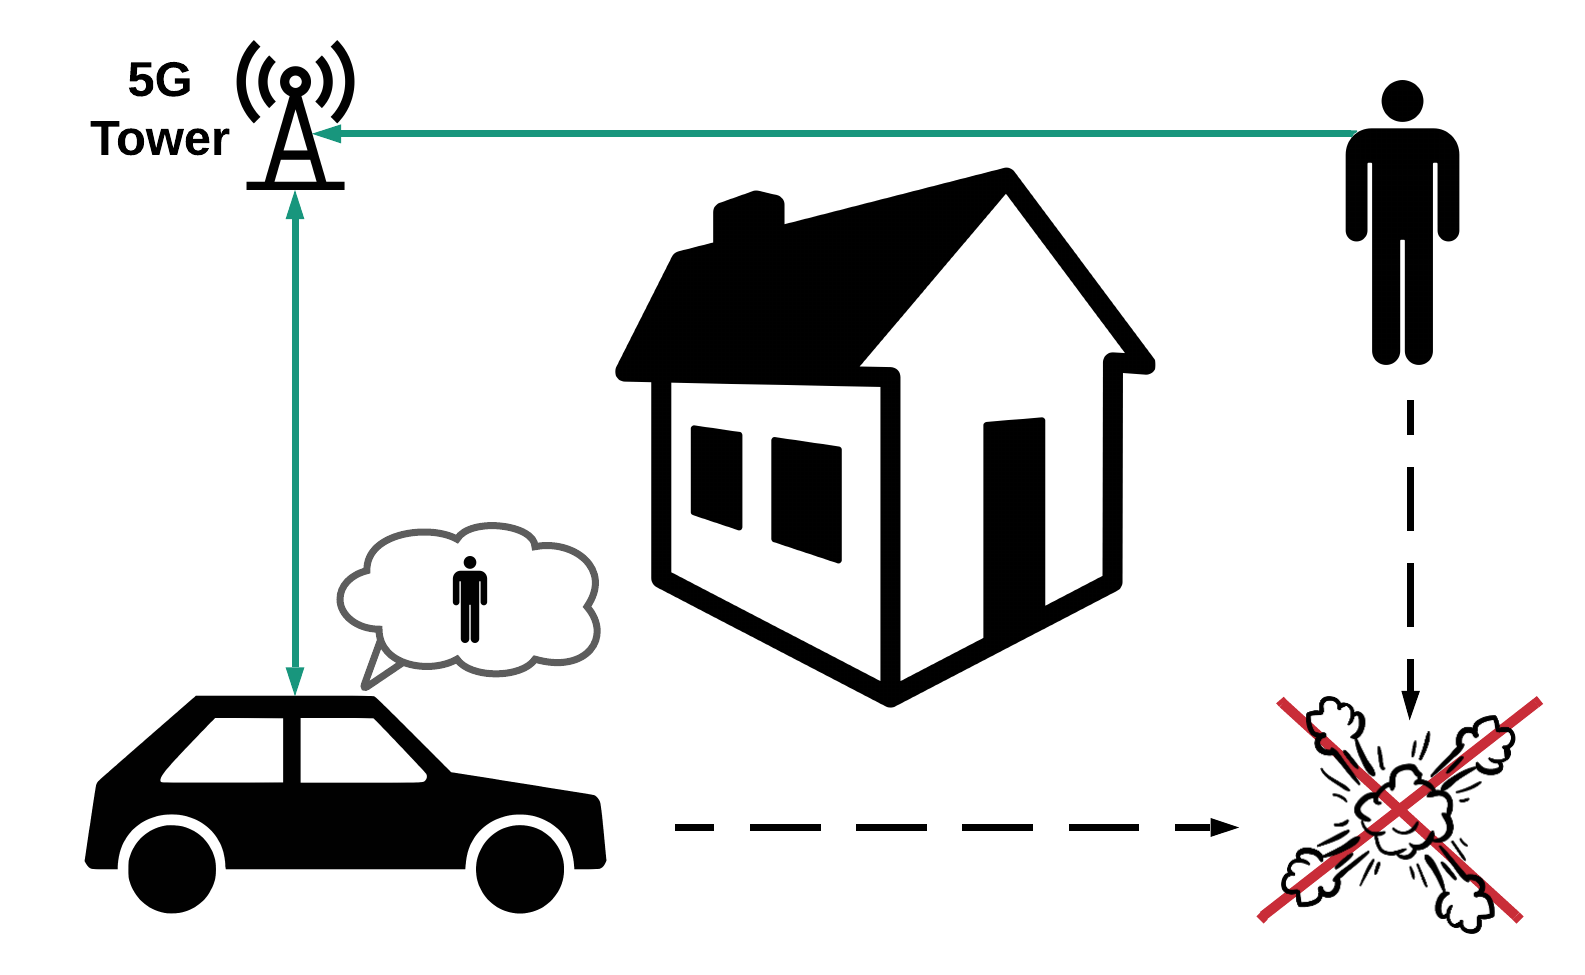
\includegraphics[width=8.5cm]{./pics/Corner.png}
    \caption{Direct signaling blocked by a building}
\end{figure}

Our protocol enables reliable, fault-tolerant transmission of the current position of traffic participants and warnings of collisions predicted from this data.

Thereby the driver and also the car itself can be notified in time of pedestrians with an Archangel-protocol-capable mobile device who are likely to cross their path in the future, based on the predicted data.

Important to highlight the main prerequisite for the operation of our system: the devices of the parties involved in traffic situations (self-driving car, mobile phone) must be 5G capable devices that support the Archangel protocol.

Technical details:

The essence of the system is that cars and pedestrians constantly share data about their position and state of motion. These data run into so-called computational units located in the middle of the zones defined by a finite number of 5G towers, which are able to predict routes and possible collision points from the data sent by the nodes (mobile phone, car). The system is capable to rank the computed information, thus prioritizing the potential collisions. Exceeding a dynamic threshold set by the system, the car is notified that a pedestrian is nearby and a potential collision is preventable.

The need of computational units is confirmed by the fact that endpoints (pedestrians and cars) alone do not have sufficient resources to process such a large amount of data. Respectively, due to the limited range of direct communication, no information would be available about points outside the communication distance of each node. We also need to take into account the case where many people or cars gather at a given point. In this case, communication between endpoints is extremely cumbersome. To remedy these problems, we introduce a centralized point into the system that has high computing capacity and is able to provide all important computations within critical time constraints with high precision, which could be considered as one source of truth in the system. The problem of many devices in a small space is eliminated by the use of network communication, including beamforming technology.

Most of the communication works through 5G, in practice, the nodes send the data to the 5G towers and the towers to the local computational unit. The most important is the area described by a given computational unit, since within this area it provides the cars with the exact already ranked notifications calculated from the processed data and thus the cars are ultimately informed of the potential danger.

\begin{figure}[h]
    \centering
    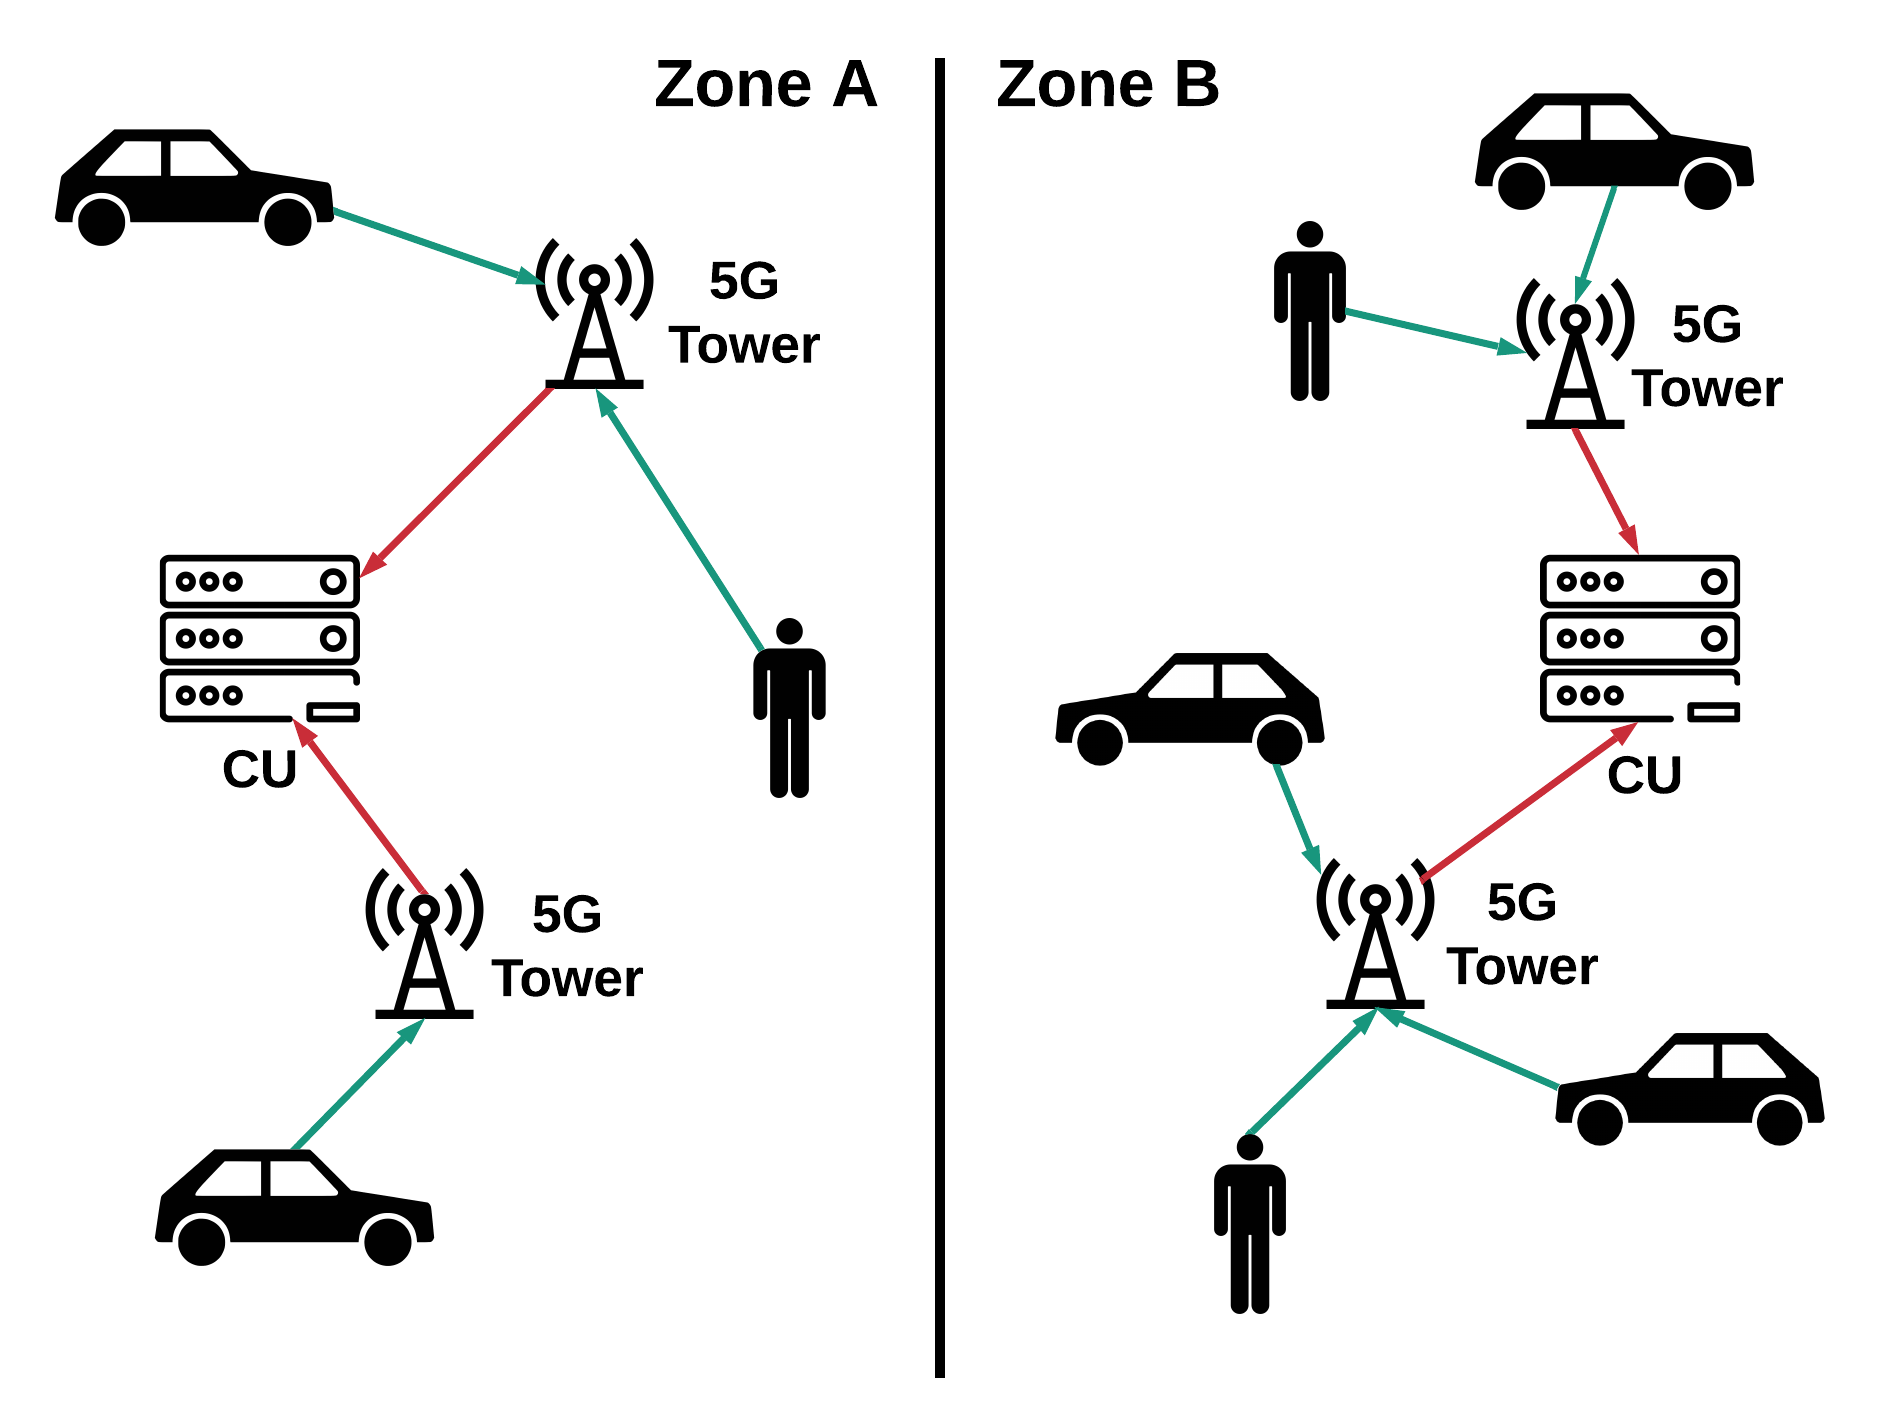
\includegraphics[width=8.5cm]{./pics/Communication.png}
    \caption{Communication inside zones}
\end{figure}

However, it is important to look at edge cases. For example what happens when a pedestrian and a car falls into a separate computational zone, even though they are close to each other. As long as the pedestrian and car computational units are able to calculate the predicted speed and direction of both separately, it is not clear whether the two objects would not cross each other, causing a potential collision. In this case, the neighboring computational units share data on the status of the pedestrian and the car. In such cases, it is obvious that the car’s computational unit needs to know the pedestrian’s data out of the other zone, as it transmits this data to the car, whether the pedestrian is now dangerously close to the car or not.

\begin{figure}[h]
    \centering
    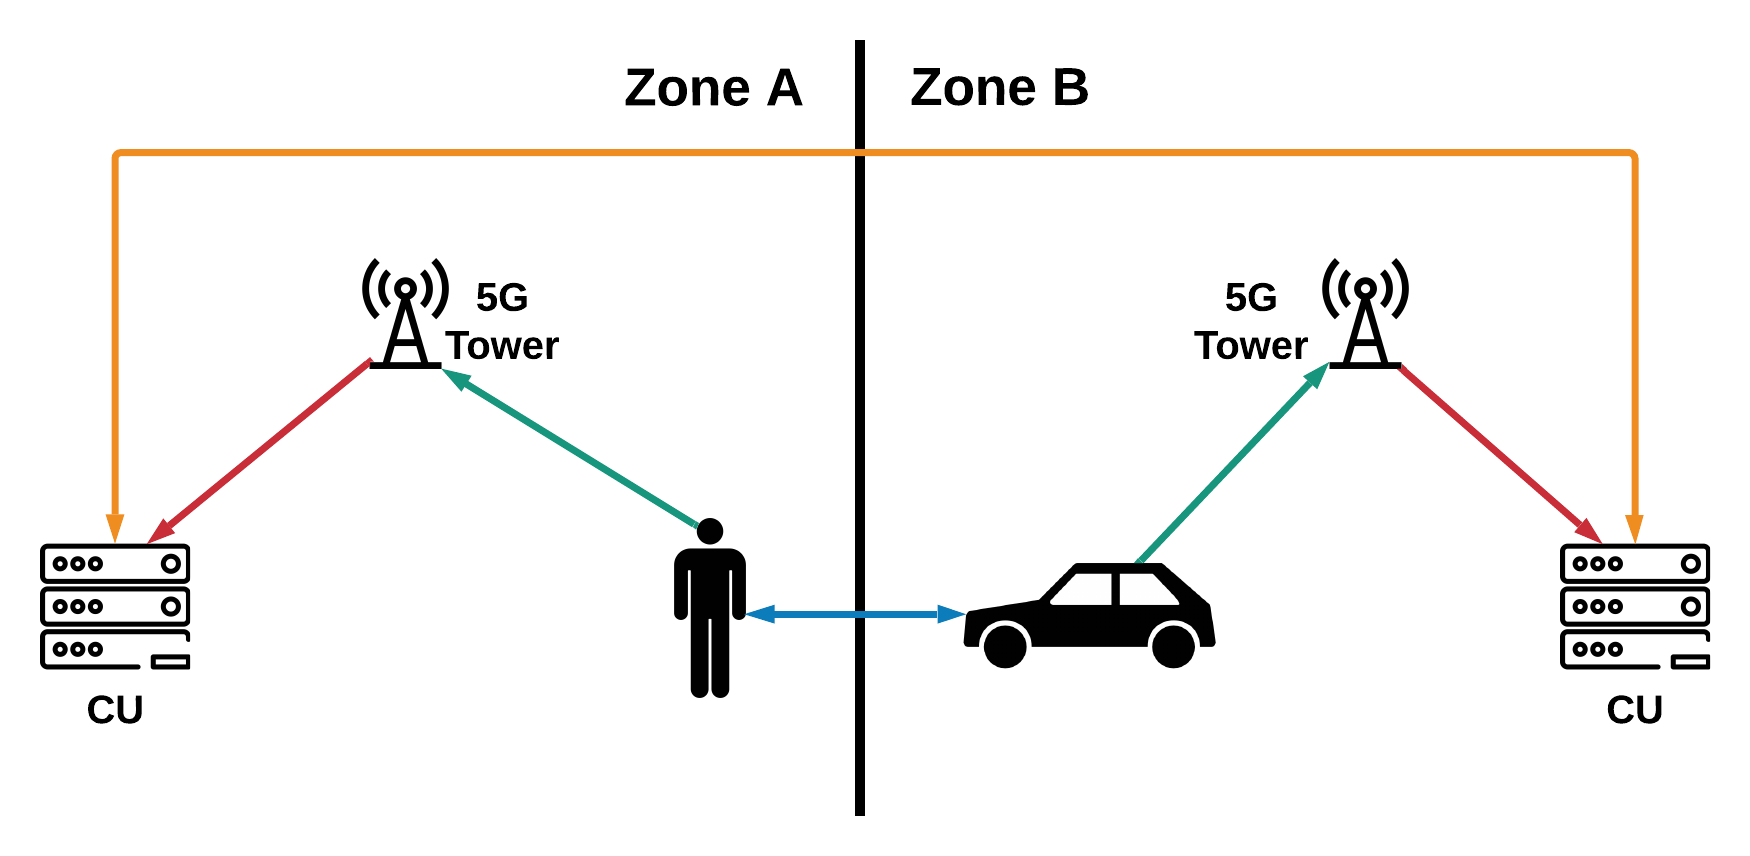
\includegraphics[width=8.5cm]{./pics/Edge case.png}
    \caption{Edge case}
\end{figure}

However, the question remains that which of the two computational units should calculate the data to be sent to the car. As far as the calculation goes the optimal case would be that the computational unit which is in the zone of the car does the computation. After all, it will ultimately notify the car, so practically we would add extra pedestrians to the area that it manages. However, we should investigate the case that what happens if the computational unit of the car’s zone is already critically loaded with computations until the pedestrian's is fully capable for the work because it is less loaded. One computational unit knows its own loadness and even knows its neighboring computational units statuses, thus it can decide that the computing or the network round trip time takes more time. If the networking scenario is chosen then the system transmits the raw data of both the pedestrian and the car to the computational unit in the pedestrian's zone, and after the calculation performed there, it returns the data to the computational unit in the car’s zone, thus balancing the load on the system. This obviously comes with extra network traffic, but since these predictions require a lot of computation, the system will choose this path if overall it would really speed up the data processing, thus saving time in general.

\section{Scoring system}

Some data is prioritized over others when sent out from the computational units. Therefore, a scoring system is introduced. Every message has a score that represents its urgency - the higher the score, the sooner the message must be sent out. The purpose of this protocol is to make the pedestrians’ life even safer next to self-driving cars. Because of this, the messages concerning pedestrians who are potentially in the most danger need to be prioritized.

Every message gets a score that describes the hazard factor of the situation. Each situation is composed of two elements: the self-driving car's movements and the pedestrian's movements. From these, the computational units calculate the points that determine the order.

A self-driving car and a pedestrian (objects of movement) need to provide the same type of data for these calculations.

The three main aspects that are taken into consideration: the speed and the direction of the movement combined with the objects’ current position. These are core factors - without them computations are not possible.

The car's and the pedestrian's positions determine their distance from each other as the crow flies. If they are closer to each other, then a change in their course could highly increase the chance of an accident. Firstly, the score is the multiplicative inverse of the calculated distance in meters.

Then from the speed and the direction, a movement vector is defined for each participant. If they are moving away from each other, the score is multiplied by (-1), so it will be the additive inverse of the original score.

If the participants' line of movement intersects with one another, then their possible meeting point is determined based on the movement vectors. The meeting point is the point in space, where - given their current speed and direction - the car and the pedestrian will reach at the same time. The time (in which they will reach that point) is taken in seconds and its multiplicative inverse is added to the score. If they will not meet, nothing is added to the score.

\begin{figure}[h]
    \centering
    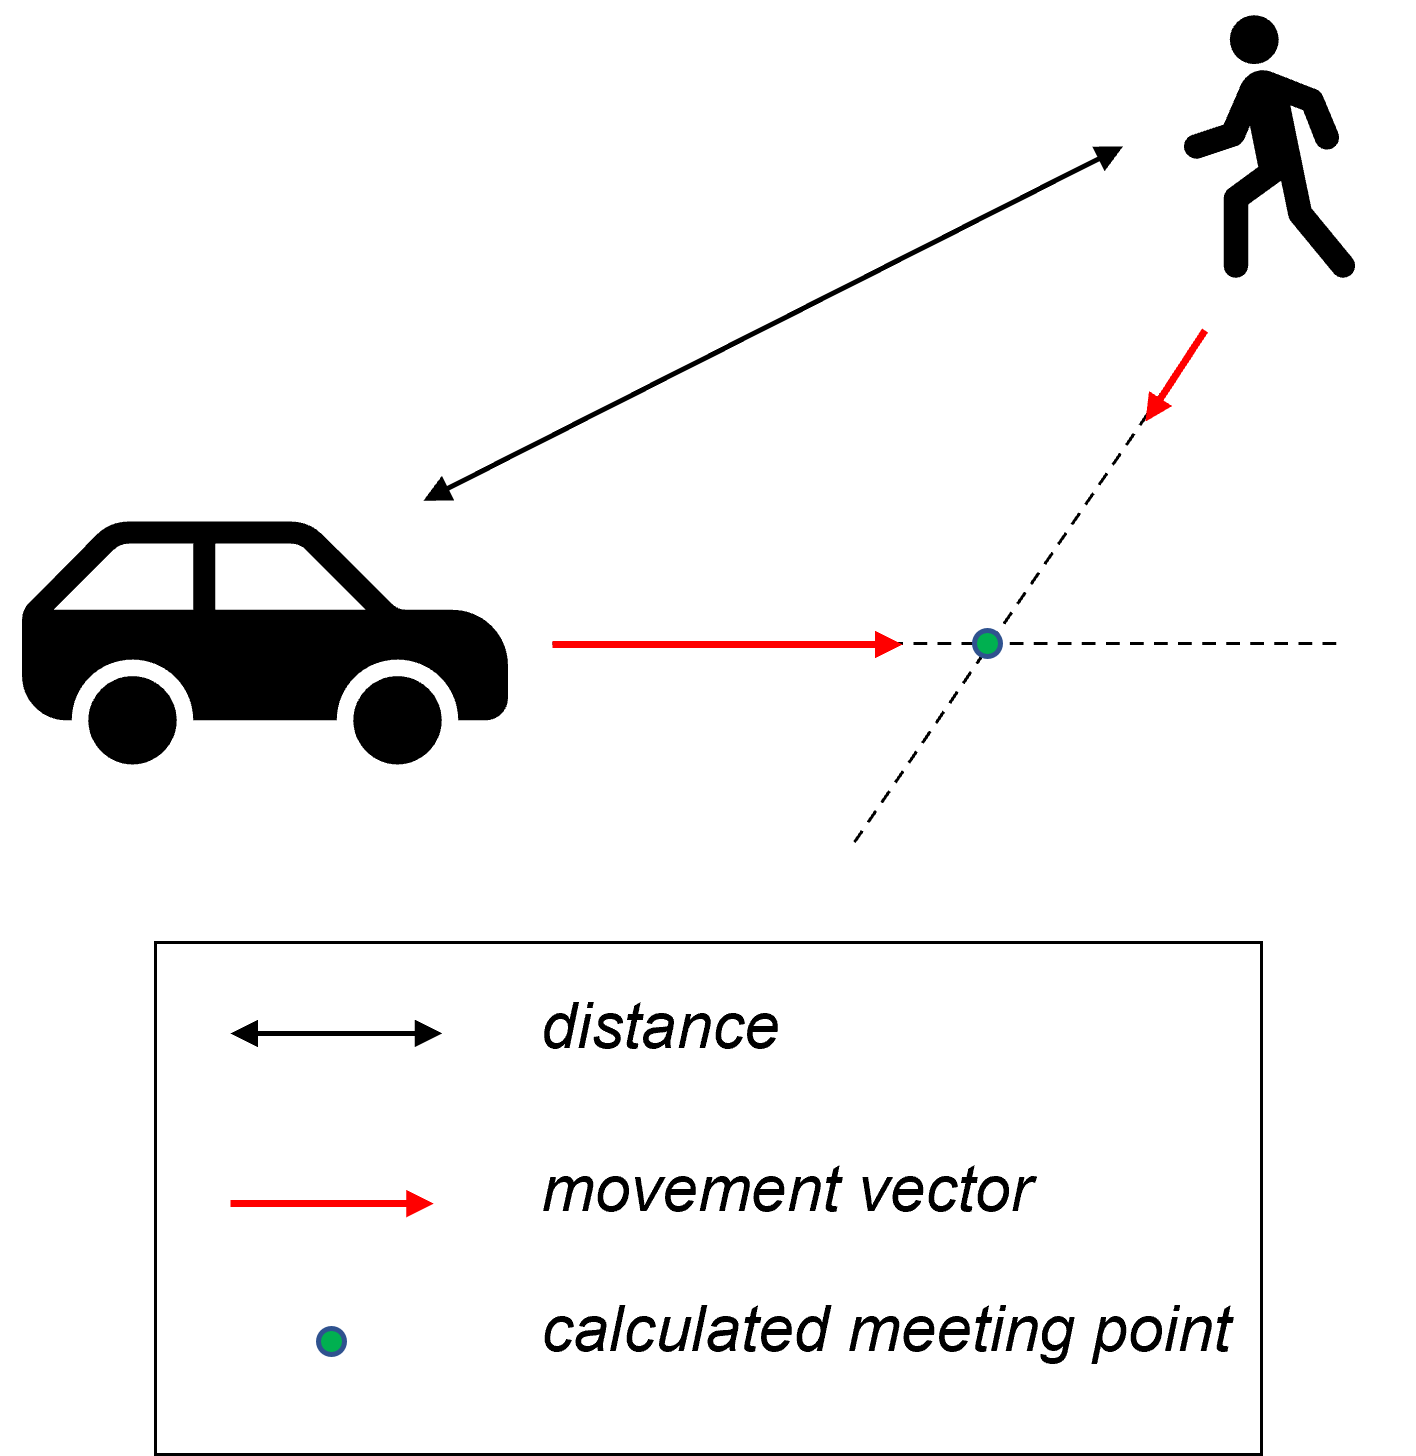
\includegraphics[width=8.5cm]{./pics/Core factors of the calculation.png}
    \caption{Core factors of the calculation}
\end{figure}

Then the environment is taken into consideration too - if there is data available. For example, if the person is in a building, then the chance of an accident is very low, but if they are on the sidewalk or walking on the road, the danger might be much higher, which the previous calculations don't show.

If there are no objects between the car and the pedestrian, then the score is multiplied by 1.5, if the pedestrian is walking on the road (instead of the sidewalk), the score is multiplied by 2. These calculations indicate the greater risk.

For every obstacle in the way of the car - which would most probably stop it before an accident could happen, therefore the walking person is safer - the score is multiplied by 0.9. These obstacles could be traffic lights, road closures, or even police officers who are conducting the traffic.

If the person’s position is inside of a building, the score is multiplied by 0.7. The position might be inaccurate thus it is not sure that the person actually is in the building. Because of that, it is not entirely safe to drop the message in this case, but its importance may be lower.

The last part of the score calculation is to assess the possibility of the routes. For example, if some information is available about the pedestrian's or the car's usual movements, it can be used to raise the scores. If a person takes the same route almost every day (for example going home from work), they likely are going the same way. If the meeting point is on a frequently taken route, then the score is multiplied by 1.5.

If a score is negative, the danger for the pedestrian - in that given situation - is minimal. That means that the message can be safely dropped. Since the probability of an accident in that specific situation is very low, it is not necessary to send out this particular message, because it would only generate surplus data traffic.

\section{Package structure}

The communication between people and towers as well as cars and towers is achieved by sending data packages. It is necessary to identify and distinguish the owners of the packages. This is solved using universally unique identifiers, or UUID as the first part of the packages.

UUID is a standardized, 128-bit label to recognize and differentiate between objects in a system therefore it can be used for unique identification. The uniqueness of the UUID is mathematically guaranteed meaning the probability of two UUIDs matching is so close enough to zero to be negligible. This is because of the vast number of possible UUIDs counting $2^{122}$.

UUID are represented as 32 hexadecimal digits, displayed in five groups separated by hyphens, in the form 8-4-4-4-12. There are different variants of UUID based on their generation method. In our work, we use the version 4 UUID, which is generated using random numbers. An example for UUID: 123e4567-e89b-12d3-a456-426614174000.

The second part of the packages is the serial number. This will be incremented at each transmission. The purpose of using serial numbers is to determine which packages need to arrive first. This helps to prioritize the packages based on their importance. The handling of high priority packages are more important than of low priority packages.

In the package after the UUID and the serial number comes the number of the datatype (code or compressed data). And finally, there is the actual data that contains all of the essential properties of the user.

These properties contain for example the user’s location, direction, velocity, activity (whether the user is walking, jogging, running, etc.). And on routes that the user takes often (from home to school/work, regular sport activities) the data is more accurate because the expected route and activity duration can be calculated beforehand with a high possibility. This helps the self-driving cars to prepare before the user even gets there.

This calculated data can be sent in two ways. One is with codes and the other is with compression.

The code type requires premade codes for each possible activity, direction, location, etc.
For example:

\begin{itemize}
    \item Activity “running”: 102
    \item Direction is south-southeast: 253
    \item Velocity is 3 meters per second: 003
    \item Location is the actual coordinates
\end{itemize}

Of course these are not essentially three digit numbers, these are just for the example.

The compressed data type is the other option. Here a fast compression is necessary. This compressed data would be sent and the receiver would decompress it to get the information.

Deciding which type is used in which scenario would be handled by an algorithm that would analyze whether the code or the compression is better. If we want to send lots of data compression is chosen while in some cases it would be a waste of resources, there the code type should be chosen. The result of this decision is the number of the datatype at the beginning of the package (after UUID and serial number).

\begin{figure}[h]
    \centering
    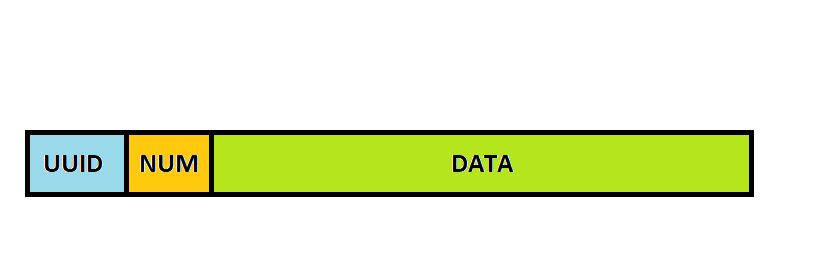
\includegraphics[width=8.5cm]{./pics/Package structure.png}
    \caption{Package structure}
\end{figure}

\section{Summary}
Even though self-driving cars don't have a long history, this branch of technology is certainly important and is far from its final form. There are still lots of problems waiting to be solved because self-driving cars are an inevitable part of the future. In our work, we managed to specify a new communication protocol which does pioneer work in protection of pedestrians. We think our work is worth the effort since traffic safety is one of the most important problems but now it is one step closer to be solved.

\section*{Acknowledgment}

The preferred spelling of the word ``acknowledgment'' in America is without
an ``e'' after the ``g''. Avoid the stilted expression ``one of us (R. B.
G.) thanks $\ldots$''. Instead, try ``R. B. G. thanks$\ldots$''. Put sponsor
acknowledgments in the unnumbered footnote on the first page.

\begin{thebibliography}{00}
    \bibitem{b1} I. Vourgidis, L. Maglaras, A. S. Alfakeeh, A. H. Al-Bayatti, M. A. Ferrag ``Use Of Smartphones for Ensuring Vulnerable Road User Safety through Path Prediction and Early Warning: An In-Depth Review of Capabilities, Limitations and Their Applications in Cooperative Intelligent Transport Systems'' Sensors 2020, 20(4), 997 - February, 2020.
    \bibitem{b2} Charles McLellan, ``What is V2X communication? Creating connectivity for the autonomous car era'' Topic: Autonomous Vehicles and the Enterprise, Part od a ZDNet special Feature - November 2019.
    \bibitem{b3} E. Ali, M. Ismail, R. Nordin, N. F. Abdulah, ``Beamforming techniques for massive MIMO systems in 5G: overview, classification, and trends for future research'' SpringerLink, Frontiers of Information Technology \& Electronic Engineering  (ISSN 2095-9184) - June 2017.
    \bibitem{b4} Stephen Shankland, ``5G could make self-driving cars smarter and commutes safer'' CNET, A RED VENTURES COMPANY - Augugust 2019.
    \bibitem{b5} Florian Sheck, Andreas Form, Axel Freyberg, ``5G: a key requirement for autonomous driving—really?'' Kearney, Communications, Media and Technology - April, 2020.
\end{thebibliography}
\vspace{12pt}

\end{document}
